\section{The research question}
\label{sec:question}
The visual drama of an approach is an unreliable guide to its mathematical difficulty. A steep-looking turn may be compatible with the aircraft's operating envelope, while a visually gentle path may consume too much distance or require an unsustainable speed change. At Kai Tak, the more useful question is how the constraints fit together: where the aircraft can turn, how much height it can lose, what state it must reach at the runway, and how much runway remains after touchdown.

The phrase \emph{Kai Tak paradox} is used here as a project framing, not as an established named theorem or a claim that historical operations violated a physical bound. It refers to the apparent tension between a constrained-looking approach and the existence of flown trajectories through it. The research task is to replace that impression with a precisely defined feasible set and a fair comparison.

Let $\theta$ collect aircraft configuration, initial conditions, environment and information assumptions, and let $\mathcal F(\theta)$ denote the admissible trajectories or policies under those assumptions. Three questions follow. Is $\mathcal F(\theta)$ nonempty? Are documented historical observations consistent with the model and its uncertainty? Does a candidate improve a specified criterion relative to a comparable baseline? These questions require different evidence. A constructed feasible path answers the first within its model. A measured flight can challenge the model. A strict, verified improvement over one baseline says nothing by itself about global optimality.

An entire published procedure should not be treated as one observed curve. Pilots can fly different trajectories consistent with a procedure, with different aircraft states and weather. Similarly, a recorded path does not identify the pilot's complete feedback policy: it reveals one response to one realized sequence of conditions. This distinction will matter when uncertainty is introduced.

\subsection{Scope of version 2}
This version develops a research benchmark and reports the results that have supporting artifacts. It uses 1993 as the main historical reference, while retaining other source epochs explicitly. It presents the retained calm-air candidate and a new candidate conditioned on the report-stated mean wind, each with its own restricted certificate. The historical reconstruction is not yet a clearance constraint in either calculation. The new wind input connects the evidence to a declared scenario without making it a reconstruction of the actual flight.

The distinction is substantive. The synthetic model is useful for testing equations, understanding coupling and verifying a candidate continuously in time. It is not a substitute for the historical problem. Conversely, an increasingly detailed reconstruction does not by itself determine aircraft dynamics or identify the best approach. Both components must eventually meet in a common coordinate system with defensible uncertainty.

\section{Historical evidence and the comparison it permits}
\label{sec:evidence}
\subsection{The primary historical anchor}
CAD Report 1/95 concerns the Boeing 747-409B B-165 operating CAL605 on 4 November 1993 \cite{cad}. Sections 1.8--1.10 describe the instrument guidance and runway; Appendices 1, 11 and 12 preserve the approach chart, selected recorder plots and a reconstructed flight path. The report supplies a coherent primary reference for the chosen period, rather than a composite of charts from different years.

The reported localiser direction is $088^\circ$ magnetic and the runway direction is $135^\circ$ magnetic. Their difference is $47^\circ$. The glidepath is reported as $3.1^\circ$, and the instrument segment ends at the middle marker, 1.7 nautical miles from touchdown. The runway is reported as 3,331.5 metres long and 61 metres wide, with 2,786 metres of landing distance available. In the threshold-relative stopping calculation, the latter is the relevant length. Total pavement length cannot silently replace it.

The magnetic difference does not establish a 47-degree air-heading change under arbitrary wind. Ground track, air heading and their coordinate references must remain separate. Nor should the missed-approach warning in the chart be converted into a universal instruction for where every landing turn begins. That warning concerns terrain clearance along the specified missed approach.

\begin{table}[H]
\caption{Selected inputs and their evidential roles. The source-based entries do not calibrate the complete aircraft model.}
\small
\begin{tabularx}{\textwidth}{@{}>{\raggedright\arraybackslash}p{0.24\textwidth}>{\raggedright\arraybackslash}p{0.24\textwidth}>{\raggedright\arraybackslash}X@{}}
\toprule
Quantity & Value or description & Role in this paper\\
\midrule
Aircraft configuration & 747-409B; four PW4056 engines; flaps 30 & Historical anchor from CAD report.\\
Landing weight & 525,718 lb, estimated in report & Source estimate; exact unit conversion does not remove estimation error.\\
Reference / case target speed & 141 / 153 kt CAS & Reported case information; CAS-to-EAS approximation is a model assumption.\\
Landing distance available & 2,786 m & Historical runway quantity used as the scenario stopping limit.\\
Initial position & $(-2500,1000,140)$ m & Synthetic runway-relative state, not a recovered flight position.\\
Wind scenarios & Calm; steady $070^\circ$ true / 21 kt & Calm reference and report-conditioned mean-wind assumption; neither recovers gust history.\\
Braking law & 2 s delay, then $0.15g$ & Fixed illustrative model, not certified runway performance.\\
\bottomrule
\end{tabularx}
\end{table}

\subsection{What the recorder evidence can establish}
The report describes a recorder containing 269 parameters, but publishes only selected plots. Those images are not raw machine-readable flight data. Digitization can recover approximate curves if axis calibration, trace thickness, overlapping lines and time alignment are handled explicitly. It cannot recover missing sampling metadata or turn a thick raster line into a high-precision measurement.

Several variables also require careful interpretation. Cockpit control-wheel, control-column and pedal positions are not automatically aerodynamic surface deflections. Thrust-lever angle was not recorded. Engine indications therefore cannot be relabelled as directly observed throttle inputs. The Appendix 12 flight path was reconstructed by integrating accelerations; comparing it with those same accelerations is a consistency check, not independent positional validation.

Most importantly, the report's discussion of touchdown does not support a causal claim against the geometry of the approach. Section 2.6.5 describes a controllable touchdown and states that touchdown parameters were not a causal factor in the accident. The approximate touchdown station and groundspeed reported there are evidence about that case, not proof that an alternative turn would have prevented the overrun. This paper treats CAL605 as an informative reconstruction benchmark, not as the historical optimum or a representative normal flight.

\status{The primary report and a verified exploratory benchmark are available. The benchmark digitizes selected flight traces and transcribes the five-sensor weather printout. It does not recover raw DFDR, a complete georeferenced flight path or an identified flight/wind clock offset. Section~\ref{sec:weather} reports the supported conditional findings.}

\section{Reconstructing the approach area through time}
\label{sec:geometry}
\subsection{A dated reconstruction, not a timeless city}
The relevant obstacle set is the city at a stated time. A modern polygon with a construction-related record does not necessarily reproduce its historical footprint, roof or surrounding ground. Demolished structures are particularly difficult to recover from a database containing only current buildings. Absence from such a database is not historical absence.

The acquisition assembled 227 valid historical survey-map archives across 93 core sheet locations and 48 full aerial frames, alongside a wider index of available sources. Registration uses the survey rasters and their supplied world files, with printed-grid checks for selected sheets. Metadata agreement establishes a coherent coordinate transformation; the raster sampling interval is not an estimate of ground accuracy. Historical map editions and photograph dates remain separate evidence.

The modern terrain and building layers provide context, not a replacement for history. The Lands Department's 5-metre terrain product documents photography from 2014--2015 and a March 2019 revision \cite{dtm}. A September 2026 building release is a different epoch \cite{buildings}. Roof and base fields are approximate elevations above Hong Kong Principal Datum. A roof elevation is not a height to be added to terrain, and Hong Kong Principal Datum must be reconciled with the aviation height reference before clearance calculations.

\subsection{What has been recovered from the 1993 photographs}
Two overlapping frames, A36142 and A36143, dated 2 November 1993, support an actual image-based stereo reconstruction. The retained result has 1,318 sparse matched points and 171,307 filtered dense surface points. Camera labels and scan-scale assumptions supply provisional intrinsics. Matched image features determine relative geometry; manually interpreted ground features and survey-road controls anchor a local metric transformation.

The vertical coordinate measures height relative to a fitted park/road plane. It is not an absolute surveyed elevation or necessarily the height of a roof above that building's own base. Two inspected roof features have conditional relative-plane estimates of approximately 10.77 and 19.20 metres. They are different features. Variation under selected focal-length and principal-point perturbations is a sensitivity experiment, not a comprehensive error interval.

\begin{figure}[H]
\centering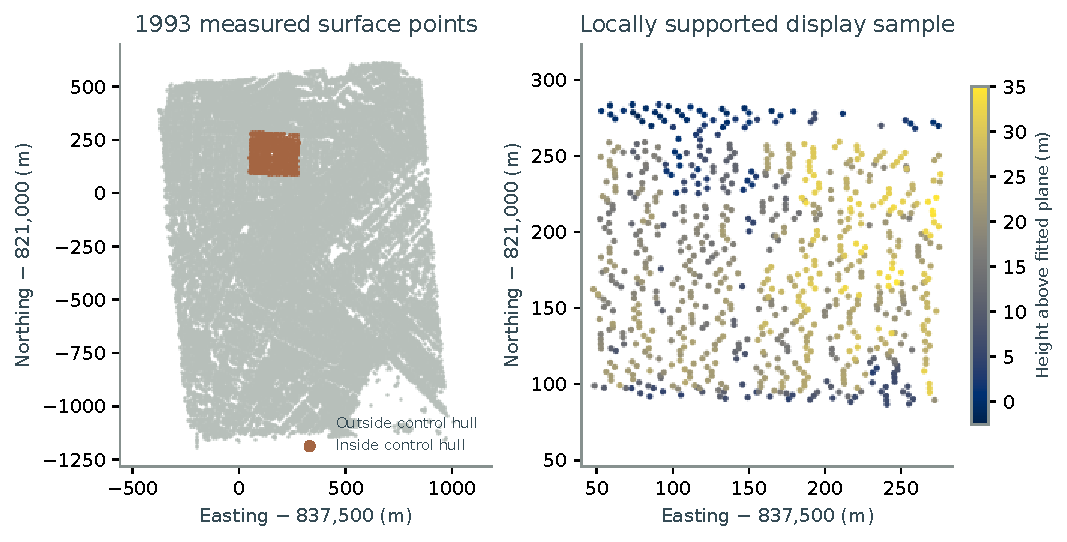
\includegraphics[width=\textwidth]{figures/historical_support.pdf}
\caption{Local support in the historical stereo point cloud. Left: deterministic every-fifth display sample of source points, distinguishing points inside the map-control hull from extrapolated points. Right: relative-plane elevations of the within-hull display sample. Coordinates are diagnostic HK1980 Grid positions with stated offsets; the vertical coordinate is not HKPD. Surfaces are unclassified. No missing region is represented as clear airspace. Source: project reconstruction of Lands Department frames A36142/A36143, 2 November 1993.}
\label{fig:stereo}
\end{figure}

The held-out map controls give a horizontal root-mean-square discrepancy of 5.754 metres for the metric stereo alignment. Only 3,780 dense points lie inside the map-control hull. These facts limit the interpretation of a visually extensive cloud: image coverage is much broader than locally controlled geometry. Points can represent roofs, ground, vegetation or mismatches that survive the filters. They do not constitute a classified, watertight city model.

\subsection{Blockwise evidence added in version 2}
Four precisely delimited road cells now have paired 1989/1994 overlays. Within them, 202 current building templates receive 404 dated assignments, and 531 dated map-region assignments form 397 cross-date geometric overlaps. The parent verification independently recomputed areas and containment for all 935 assigned geometries and checked 41 package hashes. Eight hash-linked visual observations record differences in construction, symbols and names.

These counts describe matching candidates and review units. A current template intersecting two dated maps does not prove a building persisted unchanged; a map-region overlap does not establish identity. Nor does bracketing 1993 by 1989 and 1994 editions fix a demolition or completion date between them. The supplement improves the ability to audit change, while preserving missing historical heights and unresolved identity decisions. New labelled, north-up reconstruction views improve interpretation but add no measurement accuracy.

\subsection{From surface evidence to aircraft clearance}
Clearance concerns the aircraft's swept volume and its tracking uncertainty. It cannot be established by checking a single point against a visually plausible surface. Historical building identities, roof geometry, terrain changes, occlusions, datum offsets and registration errors must be reconciled over the relevant corridor. Unknown geometry must remain unknown rather than becoming an empty obstacle list.

A conservative observed-surface mesh now connects supported points into 225,371 triangles using 155,891 vertices. It retains holes and has 86,061 boundary edges; it is not watertight. An interpolation-support correction removed 49 previously exported dense points before the geometry used in this draft was frozen. The point counts and figure reflect that corrected delivery. Neither connected triangles nor an attractive rendering establish complete building solids.

The useful intermediate output is an evidence-linked reconstruction in which each object or point records its source date, coordinate meaning and support. Such a resource allows errors to be inspected and corrected. The mathematical landing model can consume it only when the geometric assumptions required by that model are justified.

\status{Dated registered maps and conditional local stereo geometry are available. A complete historical obstacle surface with independently defensible vertical accuracy and whole-aircraft clearance is not established.}

\section{A coupled approach-to-stop model}
\label{sec:model}
\subsection{Why the phases must be considered together}
Turning, descending and slowing compete for time, distance and force. At a given airspeed, tighter turning generally raises lateral force demand. Extending the airborne path can change where the aircraft reaches the runway and how much flare distance is needed. Touchdown speed then enters the stopping law quadratically. An approach model that ends at threshold capture omits part of the constraint interaction.

The current research model uses a coordinated three-dimensional point mass. Its aircraft identity is historically anchored, but its drag, lift, thrust, rate and braking limits are stipulated scenario parameters. It does not include full attitude dynamics, sideslip, landing-gear mechanics or a calibrated wet-runway model. These simplifications make an auditable benchmark possible; they also define the limit of its conclusions.

Let $\mathbf r(t)=(x(t),y(t),h(t))$ be position relative to the usable threshold, with $x$ along the runway, $y$ to the right and $h$ above runway level. For known constant wind $\mathbf w$, define
\begin{equation}
\mathbf v=\dot{\mathbf r}-\mathbf w,\qquad V=\|\mathbf v\|,\qquad
\gamma=\arcsin(v_h/V),\qquad \psi=\operatorname{atan2}(v_y,v_x).
\end{equation}
Inverse dynamics maps a smooth position curve into required lift, bank and thrust. The model then tests those demands against its operating limits, including bank-angle rate and thrust slew. A smooth curve can fail those tests. Appendix~\ref{app:dynamics} gives the equations and distinguishes forward numerical replay from continuous-time certification.

The baseline has zero nominal wind. Constant-wind inverse dynamics cannot be extended to time-varying gusts simply by changing the position equation: air-relative acceleration then also involves wind acceleration. Neither the calm nor the new steady-wind result claims that extension.

\subsection{An explicit trajectory family}
The airborne path has approach and flare phases. In each phase, normalized time $s=(t-t_i)/T_i$ lies in $[0,1]$, and
\begin{equation}
\mathbf r_i(t)=\sum_{k=0}^{7}\mathbf c_{ik}s^k.
\label{eq:poly}
\end{equation}
Endpoint-constrained Hermite terms and shape adjustments enforce the selected boundary states. Twelve parameters govern durations, touchdown state and interior shape. Position, velocity and acceleration match at the approach--flare join. The threshold state is an intermediate target, followed by flare, touchdown, a fixed braking delay and constant deceleration.

An explicit polynomial representation is useful because it exposes derivatives and permits interval evaluation. It is not, by itself, a closed-form optimizer. The displayed candidate is one fixed set of coefficients, not a solved function assigning a trajectory to every initial state, wind and dated scene.

\subsection{The objective and its meaning}
Let $g_j\geq0$ denote operating inequalities and let $s_j>0$ be their prescribed normalization scales. The primary criterion is
\begin{equation}
\max_{q,\eta}\ \eta\quad\text{subject to}\quad
\frac{g_j(t;q)}{s_j}\geq\eta\ \text{for all relevant }t,j,
\label{eq:objective}
\end{equation}
with structural equalities and additional hard constraints enforced separately. Here $q$ is the finite parameter vector. A secondary objective minimizes integrated squared normalized bank and rate demands within the specified tolerance of the best primary score.

The score $\eta$ is a normalized model margin. Its value depends on the chosen scales and constraints. It is not an accident probability, a distance clearance or a universal measure of safety. Individual physical margins remain necessary for interpretation. An optimizer that improves on an infeasible numerical seed has constructed a better numerical candidate; it has not outperformed a valid historical flight.

\section{What the synthetic benchmark establishes}
\label{sec:results}
\subsection{A complete feasible candidate within the stated model}
The retained continuous-time certificate evaluates the exact real-decimal candidate through outward-rounded interval arithmetic. It checks a complete cover of both airborne phases, force and rate demands, endpoint conditions and the ground rule. Its 2,502 accepted closed subintervals support a normalized margin of at least 0.0397. The obstacle set in this certificate is empty. Its corridor is a stipulated reference cloud, not a surveyed historical corridor.

\begin{figure}[H]
\centering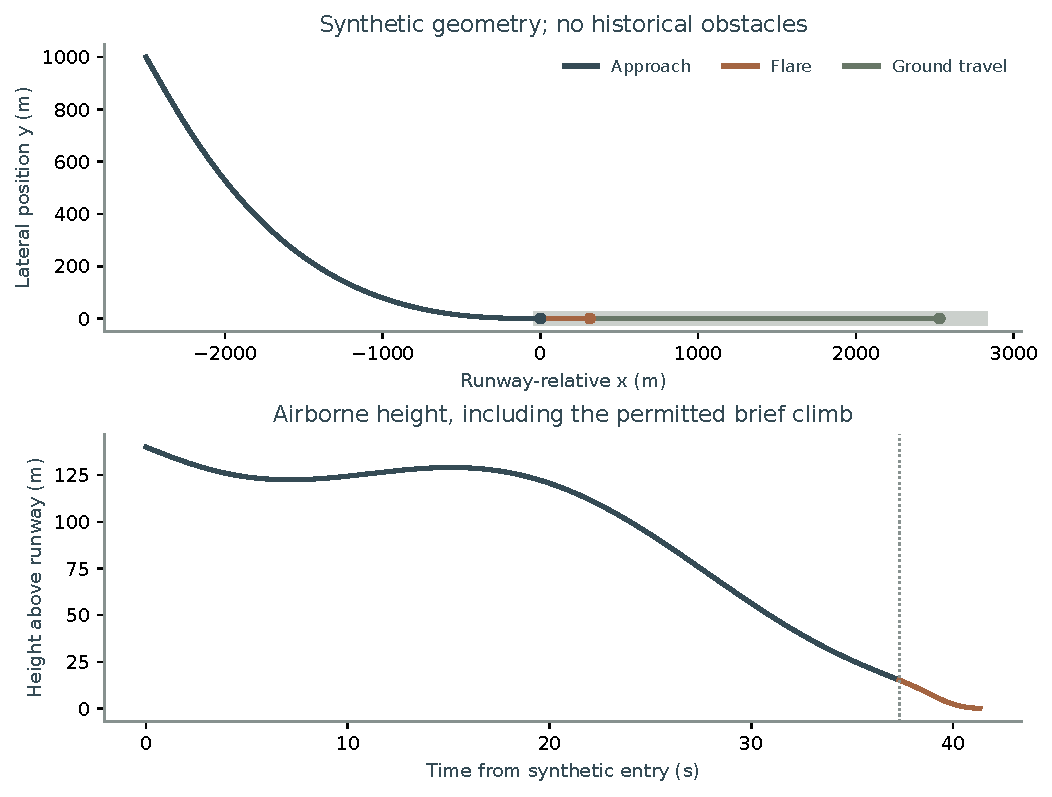
\includegraphics[width=\textwidth]{figures/synthetic_trajectory.pdf}
\caption{The explicit synthetic candidate. Plan view and airborne height are evaluated directly from the frozen coefficient export; the stopping segment uses the fixed braking law. This runway-relative frame is not geographically registered. The brief climb is permitted by the model and is shown rather than described as monotone descent. No historical terrain or buildings are included.}
\label{fig:trajectory}
\end{figure}

\begin{table}[H]
\centering
\caption{Deterministic outcomes of the fixed synthetic candidate. Rounding is for readability; no physical prediction interval is attached.}
\begin{tabular}{@{}lr@{}}
\toprule
Quantity & Scenario value\\
\midrule
Entry to threshold & 37.34 s\\
Flare & 4.00 s\\
Entry to touchdown & 41.34 s\\
Touchdown station beyond usable threshold & 313.49 m\\
Forward touchdown speed & 77.89 m/s\\
Ground travel, including braking delay & 2,217.83 m\\
Threshold-to-stop station & 2,531.32 m\\
Runway remaining & 254.68 m\\
Excess over stipulated 150 m reserve & 104.68 m\\
Entry to complete stop & 96.29 s\\
\bottomrule
\end{tabular}
\label{tab:outcomes}
\end{table}

Independent forward replay reported maximum discrepancies below $1.45\times10^{-7}$ metres in position and $4.04\times10^{-8}$ metres per second in speed. These are numerical consistency measures. They do not estimate physical aircraft accuracy, which is governed by model adequacy and calibration. Likewise, a certificate for the exact source expressions is not automatically a certificate for coefficients rounded in a printed table.

\subsection{Existence and an unresolved performance gap}
Within the specified compact parameter box, a regularity argument bounds vertical speed and excludes inverse-dynamics singularities on the positive-margin feasible domain. Continuity and compactness then establish attainment of the primary maximum. An analogous argument establishes attainment of the secondary minimum on the appropriate restricted set. These are existence results within the selected polynomial family, not formulas for the optimizers.

A separate necessary-condition argument uses the minimum flare duration, the vertical-speed bound, the minimum equivalent airspeed and the stopping constraint. It gives
\begin{equation}
0.0397\leq\eta^*<0.1559772.
\label{eq:bracket}
\end{equation}
The witness and upper bound therefore leave an absolute objective-score gap below 0.1162772. This is not a sufficiently tight result to describe the candidate as near-optimal. Appendix~\ref{app:bounds} records the argument and its domain.

Earlier tighter bounds from defective global-exclusion calculations were withdrawn. They are not used anywhere in this manuscript. Retaining that correction is important: a successful local solve, or a global search that stops with unresolved regions, cannot replace a valid upper bound. The surviving feasible witness and the independent scalar upper bound answer different questions and remain separate.

\subsection{A transparent stopping calculation}
For touchdown station $x_D$, forward speed $u$, delay $d$, deceleration $a>0$ and usable length $L$, the stipulated ground model gives
\begin{equation}
S=x_D+ud+\frac{u^2}{2a},\qquad R=L-S,
\label{eq:stop}
\end{equation}
where $S$ is threshold-to-stop consumption and $R$ is runway remaining. Differentiation yields
\begin{equation}
\frac{\partial R}{\partial x_D}=-1,\quad
\frac{\partial R}{\partial u}=-d-\frac ua,\quad
\frac{\partial R}{\partial d}=-u,\quad
\frac{\partial R}{\partial a}=\frac{u^2}{2a^2}.
\end{equation}
At the fixed candidate, an extra metre of touchdown distance removes one metre of remaining runway. The local sensitivity to a one-metre-per-second increase in touchdown speed is approximately 54.95 metres of lost runway; an extra second of delay costs approximately 77.89 metres if the other inputs are held fixed. These are partial derivatives of an illustrative stopping law, not effects estimated from accident data. The airborne trajectory may not permit the inputs to vary independently.

\begin{figure}[H]
\centering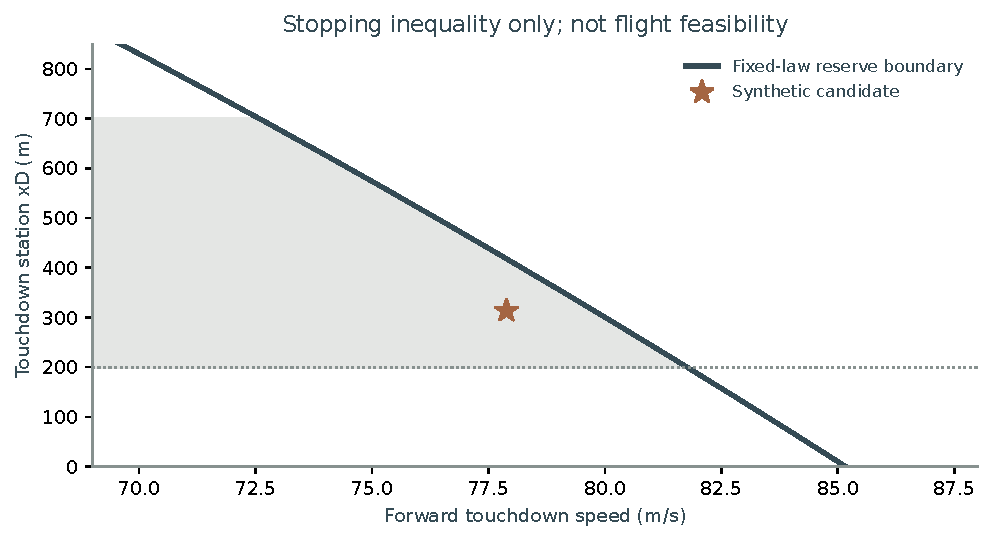
\includegraphics[width=0.93\textwidth]{figures/stopping_boundary.pdf}
\caption{Conditional stopping boundary under the fixed law. The curve shows the latest touchdown station consistent with the stipulated 150 m reserve, as a function of forward touchdown speed. Delay is 2 s, deceleration is $1.4709975$ m/s$^2$, and available length is 2,786 m. The shaded region satisfies this scalar stopping inequality only; it is not an airborne-feasibility region. The star marks the synthetic candidate.}
\label{fig:stop}
\end{figure}

This calculation illustrates why touchdown location and speed belong in the same problem as the approach. It does not demonstrate that speed can be reduced safely at any desired point, that stronger braking is available, or that a historical crew had the information and controls assumed by a counterfactual optimizer.

\section{A complete landing in the declared mean-wind case}
\label{sec:wind}
\subsection{Constructing a reference rather than fitting the accident}
The new calculation asks what the stipulated model can construct when conditioned on the report's rounded mean wind. It jointly chooses the approach, flare and touchdown parameters, then applies the unchanged stopping rule. It is not a fit to the recorded accident trajectory and does not impose the report's touchdown state as a terminal target.

The input is wind \emph{from} $070^\circ$ true at 21 kt. The chart's runway bearing of $135^\circ$ magnetic and $1^\circ50'$ west variation give the scenario axis $133^\circ10'$ true. The variation is dated 1990; using it is an explicit convention, not a surveyed 1993 runway registration. In forward/right/up coordinates the resulting constant vector is approximately
\begin{equation}
\mathbf w=(-4.87659,\ 9.64007,\ 0)\ \mathrm{m/s}.
\end{equation}
The forward component is a headwind and the rightward component is crosswind. Appendix~\ref{app:wind} gives the conversion and the case-specific bound.

The synthetic entry position, initial ground track and EAS, threshold conditions, aircraft parameters, twelve-dimensional decision box and original zero-wind reference corridor are retained. Endpoint ground velocities and inverse controls are recalculated for the wind. Consequently this is not a common full-state experiment: fixed EAS and track do not imply fixed ground velocity when wind changes. No nominal calm certificate is reused.

\subsection{The complete approach-to-stop result}
The selected solution uses 41.223 seconds to reach the threshold and 4.142 seconds in flare. It touches down 302.114 metres beyond the usable threshold at 72.490 m/s horizontal ground speed. After the fixed two-second delay, the prescribed deceleration stops it at 2,233.231 metres. The available length is 2,786 metres, leaving 552.769 metres, or 402.769 metres beyond the required reserve.

\begin{table}[H]
\centering\small
\caption{Constructed mean-wind landing. Time is measured from the synthetic entry. These are deterministic model outputs, not a recovered flight or physical prediction interval.}
\begin{tabular}{@{}lrr@{}}
\toprule
Event & Time (s) & Relevant state\\
\midrule
Synthetic entry & 0.000 & 140 m height; 153 kt EAS\\
Threshold crossing & 41.223 & 15.24 m height; 142.281 kt ground speed\\
Touchdown & 45.365 & 302.114 m; 140.909 kt ground speed\\
Braking begins & 47.365 & Fixed delay ends\\
Complete stop & 96.644 & 2,233.231 m; 552.769 m remaining\\
\bottomrule
\end{tabular}
\label{tab:windoutcomes}
\end{table}

\begin{figure}[htbp]
\centering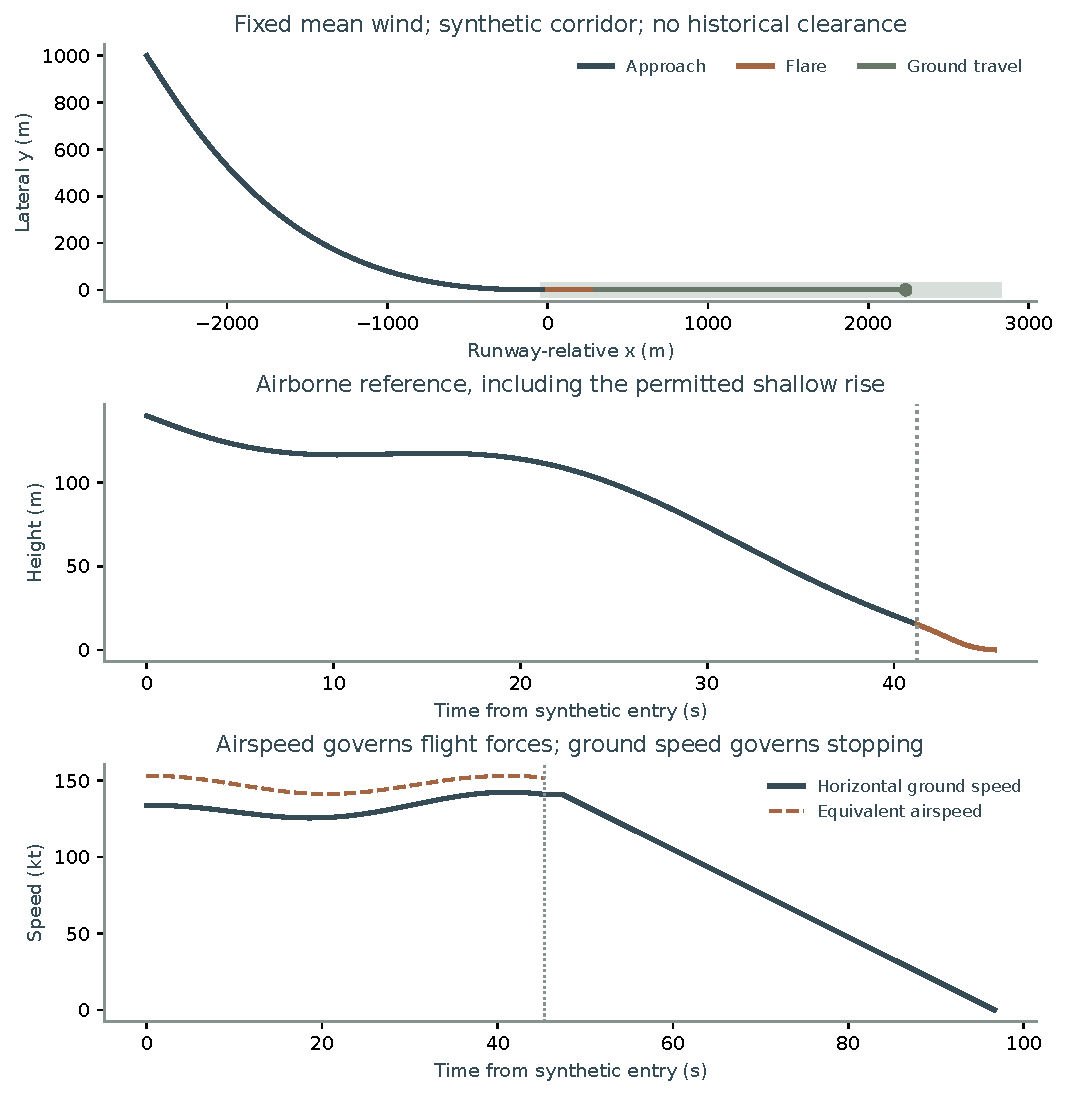
\includegraphics[width=\textwidth]{figures/wind_landing.pdf}
\caption{The new wind-conditioned reference, evaluated from its frozen polynomial coefficients and fixed ground law. The turn, height and speed profiles show a complete landing, including the shallow early rise permitted by the scenario. The ground-speed/EAS difference matters for stopping; ground aerodynamic controls are not extrapolated beyond contact. Coordinates remain synthetic and no historical obstacles enter the solve.}
\label{fig:windlanding}
\end{figure}

Maximum sampled bank is $10.421^\circ$ and maximum bank-angle rate is $2.351^\circ$/s. Touchdown EAS is 151.558 kt, substantially above its 140.909 kt ground speed. The shallow early rise is admissible because monotone descent was not imposed. It must not be hidden by describing the output as a standard approach procedure. Adding that constraint would define a different problem.

\subsection{What the numerical and continuous checks establish}
Four deterministic primary starts succeeded. A denser primary refinement and a secondary effort solve give six retained solver records. On 10,001 exact-rate samples per airborne phase, the selected minimum normalized margin is approximately 0.1527933852. The secondary solution loses approximately $5.22\times10^{-5}$ relative to the retained primary score, within the stipulated $10^{-4}$ tolerance. Agreement among local starts and a small secondary loss are not global optimality proofs.

An independent Newton integration recomputes aerodynamic forces from its integrated state. Its maximum position discrepancy is about $7.3\times10^{-8}$ m and its stop discrepancy about $4.4\times10^{-7}$ m. These values check numerical consistency of the reference and dynamics. They contain no empirical claim about an aircraft's ability to track the curve.

The stronger all-time statement comes from a wind-aware outward-rounded interval calculation at 40 decimal digits. A cover of 376 accepted closed subintervals checks both flight phases, their one-sided join rates, hard inequalities and the exact terminal/ground law. For the declared real-decimal candidate and model it supports
\begin{equation}
\eta_{\mathrm{candidate}}\geq 0.1507934696816132.
\label{eq:windlower}
\end{equation}
This certified lower enclosure is deliberately distinct from the sampled minimum. The lower value reflects enclosure conservatism; it is not an estimated physical safety factor. Its provenance binds the candidate, calculator, checker, configuration and unchanged corridor.

A separate necessary bound, derived from touchdown distance, the minimum permitted ground speed and stopping, gives
\begin{equation}
\eta^*_{\mathrm{wind}}\leq\frac{66656817}{307536544}
\approx0.2167443782.
\label{eq:windupper}
\end{equation}
Here $\eta^*_{\mathrm{wind}}$ denotes the supremum within this fixed scenario family; the zero-wind attainment proof is not silently extended. Combining the two bounds gives
\begin{equation}
0\leq\eta^*_{\mathrm{wind}}-\eta_{\mathrm{candidate}}
\leq0.0659509085084467.
\end{equation}
The right side is rounded upward from the exact rational difference. It is an absolute normalized-score bound, not a percentage performance loss. It is too wide to establish near-optimality or identify the global secondary-effort minimum.

\begin{figure}[htbp]
\centering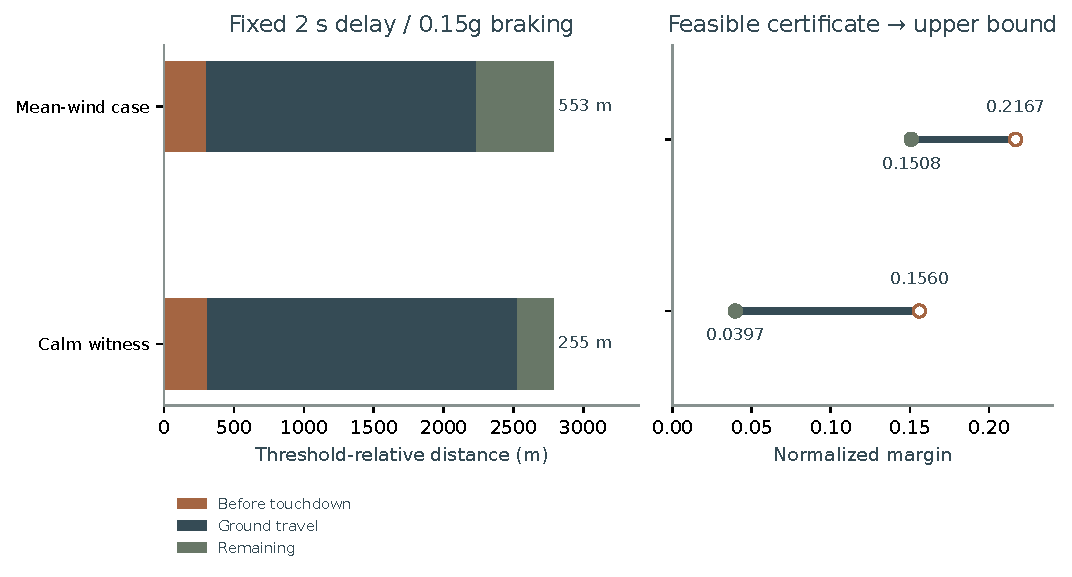
\includegraphics[width=\textwidth]{figures/scenario_comparison.pdf}
\caption{Two declared scenario problems, not a historical treatment comparison. Left: touchdown, ground travel and runway remainder under the same stopping law. Right: surviving certificate-to-upper-bound intervals for the finite-family score. The calm upper endpoint is strict; the mean-wind bound is non-strict. The lower endpoint is a feasible certificate, not the optimizer's proven value. Changing wind also changes endpoint ground velocities and the chosen curve.}
\label{fig:scenariocomparison}
\end{figure}

\subsection{Why the larger runway remainder is not historical superiority}
The new candidate leaves 298.090 metres more than the retained calm witness. In the scalar ground law, 11.378 metres come from its earlier touchdown and 286.712 metres from the difference in speed-dependent ground travel. This is an algebraic decomposition across two outputs, not a causal allocation of the benefit of wind or reoptimization. Both the operating environment and the curve differ, and neither entry state is recovered from CAL605.

The new solve therefore changes the study in a specific way: historical mean-wind information now conditions an explicit complete trajectory with its own certificate. It does not incorporate the observed gust sequence, source-supported historical obstacles, a calibrated wet-runway model or the crew's actual information set. In particular, the CAD finding that actual touchdown was controllable and not causal cannot be overturned by comparing it to this stipulated braking law.

\status{Complete conditional approach/flare/stop reference, independent force replay, all-time model-feasibility certificate and loose family gap bound are available. Historical clearance, physical prediction intervals, global near-optimality and accident-prevention claims remain unestablished.}


\section{Historical confrontation: stopping and weather}
\label{sec:weather}
\subsection{When the synthetic runway margin disappears}
The settled CAL605 benchmark contains 190 selected approach/final-phase pixel anchors, 35 speed--distance anchors and a complete transcription of the printed five-sensor A/B/C wind fields. Source overlays, extraction methods, reading sensitivities and discrepancies are retained. Its verification record reports 43 passing tests and reproduction of 19 numerical files. These establish a reproducible exploratory reconstruction, not independent physical sensor accuracy.

A direct conditional comparison substitutes the report-stated touchdown station of approximately 480 m and groundspeed of 160 kt into equation~\eqref{eq:stop}, while holding the model's 2 s delay, $0.15g$ deceleration and 2,786 m available length fixed. The results are:
\begin{table}[H]
\centering\small
\caption{Changing touchdown inputs under the same illustrative stopping law. Historical inputs are rounded report values; the rows are conditional calculations, not alternative validated flights.}
\begin{tabular}{@{}lrrr@{}}
\toprule
Inputs & Touchdown (m) & Speed (kt) & Runway left (m)\\
\midrule
Synthetic reference & 313.49 & 151.40 & 254.68\\
Later touchdown only & 480.00 & 151.40 & 88.17\\
Higher speed only & 313.49 & 160.00 & 4.99\\
Both report-stated inputs & 480.00 & 160.00 & $-161.52$\\
\bottomrule
\end{tabular}
\end{table}
Later touchdown consumes another 166.51 m; the speed change consumes another 249.69 m at fixed delay and deceleration. A negative remainder places the formula's stop beyond the runway. It does not reconstruct the aircraft's final movement into the water. The synthetic and historical entry conditions, environment and control histories differ, so this calculation cannot establish a superior approach.

\subsection{Falling speed can accompany a worsening stopping requirement}
For current speed $v$, runway remaining $R$ and assumed additional delay $\tau$, the constant deceleration needed to stop at the end is
\begin{equation}
a_{\mathrm{req}}=\frac{v^2}{2(R-v\tau)},\qquad R>v\tau.
\label{eq:required}
\end{equation}
This is a diagnostic, not the deceleration actually applied. Applying it to the report's narrative landmarks gives a rising requirement even as speed falls. With no additional delay, the requirement rises from about $0.150g$ at 2,300 m remaining and 160 kt, to $0.191g$ at 1,365 m and 139 kt, $0.221g$ at 1,080 m and 133 kt, and $0.255g$ at 880 m and 129 kt. An additional two-second delay at the last state raises the conditional requirement to about $0.300g$.

\begin{figure}[H]
\centering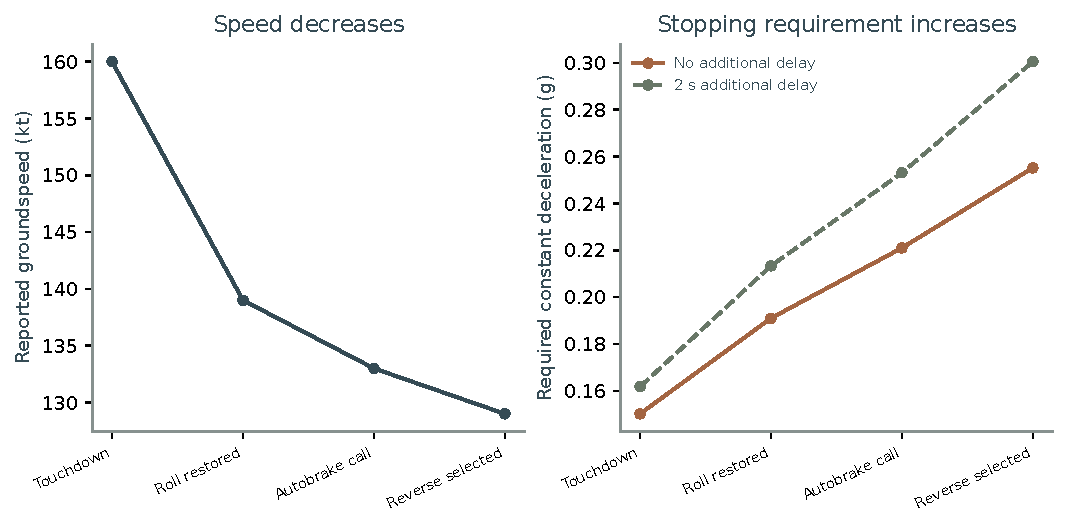
\includegraphics[width=0.96\textwidth]{figures/historical_stopping.pdf}
\caption{Source-stated CAL605 rollout landmarks evaluated through the constant-deceleration diagnostic. Reported speed falls while required deceleration rises because available runway is being consumed. The curves connect four narrative landmarks; they are not continuous measurements or fitted aircraft deceleration. CAD Report 1/95, sections 2.2.5--2.2.7; derived from equation~\eqref{eq:required}.}
\label{fig:historicalstop}
\end{figure}

The report already describes the stopping-aid sequence, including forward-thrust advancement, autobrake disarming and spoiler retraction after touchdown, followed by much later strong deceleration. The contribution here is an auditable quantitative description connected to the explicit model, not a new discovery of the accident's cause. A fixed-delay, constant-braking model does not encode those discrete states. More precise approach geometry alone will not repair that mismatch.

The source also contains different approximate touchdown-distance conventions: about 2,300 m remaining in the narrative, 2,250 m in Appendix 13 and roughly 2,210 m at the digitized Figure 5 ground-flag transition. These are retained rather than forced into agreement. Equation~\eqref{eq:required} uses the narrative landmarks; the preceding table uses $2786-480$ as the threshold-consistent remaining length. Their numerical differences are not presented as contradictory precise measurements.

\subsection{The airport wind is not a single number}
The ground-weather printout contains 15 irregular timestamps, five sensors and three A/B/C fields: 225 printed direction--speed pairs. The A field is a maximum one-second speed within a five-second window; B and C are overlapping two- and ten-minute averages. At wind-system 03:35:30, the NW sensor shows 37 kt in A, 23 kt in B and 19 kt in C. At 03:38:00, NW shows 12 kt while Lei Yue Mun shows 37 kt in A. These differences describe sensor location and aggregation window, not measured wind shear along the aircraft's path.

The ground-weather clock's offset to the flight/ATC timeline is unidentified. No exact synchronized join is imposed, and no particular ground gust is assigned as the cause of a flight excursion. The printout was event-triggered and does not contain all recorded peaks. Interpolation would add assumptions, not recover missing observations.

\subsection{Annual station-weather context}
The retained NOAA Integrated Surface Database archive contains 8,549 records for station identifiers 450070--99999 in 1993, including 24 records on 4 November \cite{noaa,isd}. Decoding preserves source flags, missing values and raw fields. A record containing missing wind is not converted to calm conditions, and absence of a gust group is not interpreted as zero gust.

For descriptive comparison, the routine subset is fixed to FM-15 reports with source flag 4, exact UTC-hour timestamps, normal-wind coding, present wind speed with quality code 1 or 5, and exclusion of rows missing both temperature and visibility. It contains 8,360 observed records. This is a selected archive subset, not a random sample of landings or a complete set of independent weather states.

The 03:00 and 04:00 UTC reports on 4 November both give wind from $070^\circ$ true at 10.8 m/s, approximately 21 knots. Their structured gust values are 17.5 and 20.6 m/s, respectively. Agreement of the mean values with the CAD published mean is cross-source consistency; the sources may derive from the same originating observations. Neither hourly value establishes the instantaneous three-dimensional wind acting on the aircraft between reports.

\begin{figure}[H]
\centering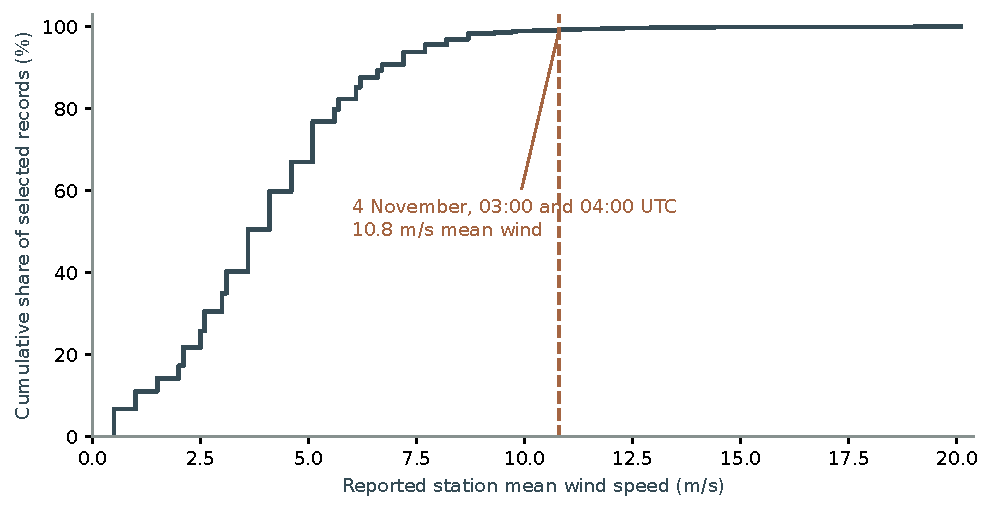
\includegraphics[width=0.94\textwidth]{figures/weather_context.pdf}
\caption{Observed routine station-wind context in 1993. The empirical cumulative distribution uses the declared 8,360-record subset. At 10.8 m/s, 8,285 records are strictly lower, 17 tie and 58 are higher. Serial dependence, missing hours and selection rules preclude interpreting the display as an accident probability, return period or distribution of aircraft-local wind. Source: decoded NOAA ISD 450070--99999 archive.}
\label{fig:weather}
\end{figure}

The case therefore challenges the model in a non-benign observed weather context. But it does not calibrate a gust process. Station siting, sensor height, the relation between surface measurements and aircraft-local wind, and clock offsets remain material. A high rank in the annual routine subset cannot identify which wind realization acted along the flight path.

The matched-case reconstruction preserves separate wind-system and flight-recorder clocks. Published narrative events cross-check digitized curves, but they are not necessarily independent measurements. Comparison to the zero-wind synthetic witness exposes the mismatched conditions rather than interpreting the distance between curves as pilot inefficiency.

\status{Selected flight-trace reconstruction, wind-printout transcription, NOAA decoding and conditional stopping diagnostics are available in the settled benchmark. A complete georeferenced trajectory, physical uncertainty calibration, routine-flight validation and an equivalent-conditions improvement comparison remain unresolved.}

\section{Uncertainty, counterfactuals and the meaning of a better approach}
\label{sec:uncertainty}
\subsection{Different errors require different evidence}
Measurement error concerns observed inputs, such as positions or a plotted speed trace. Model discrepancy concerns the difference between the chosen aircraft equations and real dynamics. Approximation error concerns a compact rule's difference from its reference computation. Tracking error concerns an aircraft's departure from the planned reference. An optimality gap concerns the distance between achieved and best admissible objective values. These cannot be compressed into one numerical band without a joint model and supporting evidence.

For example, a terrain product's stated accuracy at a confidence level does not supply a worst-case obstacle bound. An interval-arithmetic proof controls numerical enclosure under its assumptions, not the correctness of the assumptions. A held-out horizontal map-control error does not independently calibrate vertical roof error. Each number must retain the question it answers.

\subsection{What deterministic envelopes already provide}
Suppose evidence supplies a joint enclosing box for $x_D,u,d,a,L$, with positive lower deceleration and nonnegative speed and delay. Monotonicity of equation~\eqref{eq:stop} gives
\begin{align}
S_-&=x_-+u_-d_-+\frac{u_-^2}{2a_+},&
S_+&=x_++u_+d_++\frac{u_+^2}{2a_-},\\
R&\in[L_- -S_+,\ L_+-S_-].
\end{align}
These are exact extrema over the Cartesian box for the stated scalar law. Dependence or flight constraints can make the range conservative. Statistical independence is not assumed. No physical box has been calibrated for this manuscript, so the formulas do not justify attaching a numerical physical band to Table~\ref{tab:outcomes}.

A prediction interval for an individual landing requires a justified conditional distribution for the outcome and validation in the intended domain. It differs from a confidence interval for a mean or an estimated coefficient. Marginal intervals for touchdown and stopping do not automatically provide joint coverage, and endpoint coverage does not establish clearance along an entire path.

\subsection{The information available to a candidate matters}
An offline optimizer may be given an entire future wind history. A pilot or causal controller cannot use unobserved future disturbances. The distinction can be written as
\begin{equation}
\exists\pi\ \forall w\in\mathcal W:\ \text{constraints hold}
\qquad\text{versus}\qquad
\forall w\in\mathcal W\ \exists\pi_w:\ \text{constraints hold}.
\end{equation}
The second statement permits a different solution after each complete wind realization is known. It is weaker than a single admissible policy that works across the disturbance set. A fair historical comparison must specify the information set, response limitations and navigation aids as well as aircraft dynamics.

The primary counterfactual should keep aircraft, mass, entry state, runway, dated obstacles, braking, operating limits and available information fixed. A modern-guidance comparison can be useful, but is a separately labelled question. A candidate can only disprove the optimality of a particular baseline if both are feasible for the same problem and its strict advantage exceeds relevant uncertainty.

\section{Relation to existing research and contribution to Hong Kong}
\label{sec:contribution}
\subsection{Where the research sits}
Aircraft trajectory optimization, bounded-curvature planning and robust tracking are established subjects. Wu and Chen characterize minimum-time paths for a Dubins airplane in steady wind; some candidate families reduce to quadratic equations and others require transcendental root finding \cite{wu}. That reduced setting is a valuable benchmark, not a complete descending landing with flare and stopping.

Kim and coauthors study six-degree-of-freedom landing trajectories with runway alignment, obstacles and constant wind using sequential convex programming \cite{kim}. That provides a substantially richer dynamics comparator. FaSTrack separates a simplified planner from tracking dynamics and a tracking-error bound \cite{fastrack}. Its demonstrations do not certify a Kai Tak airliner, but the distinction between planned geometry and trackable motion is directly relevant here.

The present paper does not claim novelty merely from applying optimization to Kai Tak. Its prospective addition is the combination of a documented historical benchmark, explicit approximate trajectory rules, transparent performance bounds and uncertainty-aware confrontation with records. Each element must be evaluated against its own literature. The current screening is bounded rather than exhaustive, and the comparative algorithms have not been reproduced in this version.

\subsection{A useful historical research resource}
The immediate public value lies in making a difficult historical engineering problem inspectable. A dated source catalogue and reconstruction can support aviation-history teaching. An explicit model can show students why reaching the runway is not the same as completing a landing. A reproducible analysis can help future researchers distinguish a missing input from a mathematical impossibility.

The public research repository contains authored code, provenance records and explanatory visualizations, with larger source packages separately inventoried and source rights retained. It would distinguish original materials from derived artifacts and preserve gaps rather than inventing completeness. Version 2 is prepared for the authorized GitHub release alongside its editable source and frozen evidence. Public availability is not peer review, external adoption or demonstrated societal impact. Potential uses are not evidence that those uses have already occurred.

The work's relevance to Hong Kong follows from its object: the geometry, records and engineering history of a particular place. A generalizable mathematical method would be an additional contribution, not a prerequisite for a careful historical dataset to be useful. Contemporary aviation applications would require separate validation.

\section{Limitations and the next version}
\label{sec:next}
Version 2 has a wind-conditioned mathematical candidate and historical evidence, but not yet a historical candidate validated against complete terrain and aircraft data. Its central remaining task is integration under defensible assumptions. It must not close that gap by relabelling a synthetic path, replacing unknown historical obstacles with empty space, or attaching arbitrary probability distributions to uncertain inputs.

\begin{table}[H]
\caption{Evidence needed before the corresponding stronger claim can enter the paper. These are unfinished research requirements, not exclusions from the intended study.}
\small
\begin{tabularx}{\textwidth}{@{}p{0.32\textwidth}X@{}}
\toprule
Proposed claim & Required evidence\\
\midrule
Historical model consistency & Source-linked flight traces; defensible clock, speed and height conventions; explicit model comparison with uncertainty.\\
Terrain-aware feasibility & Registered runway and historical obstacle geometry; datum reconciliation; aircraft-volume and tracking allowance; full-path checks.\\
Useful condition-dependent rule & A domain wider than the single fixed mean-wind case, validated reference solutions, explicit condition-dependent coefficients and out-of-domain refusal.\\
Near-optimality & A valid, useful objective-gap bound for the same feasible set and objective.\\
Calibrated landing predictions & Supported joint input/discrepancy assumptions and relevant out-of-sample coverage evidence.\\
Historical improvement & A valid baseline and candidate with equivalent conditions and information; an advantage that survives uncertainty.\\
\bottomrule
\end{tabularx}
\end{table}

The matched CAL605 benchmark now exposes a specific limitation: a two-second delay followed by constant braking does not encode the stopping-aid history in this event. The next empirical task is to identify which dynamics and discrete states can be supported by the records, preserving the frozen baseline while any proposed model change is assessed explicitly. Broader validation remains dependent on routine approaches, go-arounds and their configuration and weather metadata.

The mathematical priority is a useful certified gap or a clearly scoped approximation result after historical constraints are introduced. Exact symbolic global optimality is not required for the intended study. An explicit approximation with honest error and performance bounds can be more informative than an opaque numerical optimum, provided its domain and limitations are established.

\clearpage
\section{Conclusion}
Version 2 advances from a calm-air feasibility example to a complete wind-conditioned mathematical landing. Its explicit curve covers turning, descent, flare, touchdown and stopping without changing the stipulated braking. The new candidate leaves 552.77 metres of runway in its scenario, and its own continuous-time certificate verifies a positive normalized margin. A valid upper bound quantifies the remaining uncertainty about the best member of the finite family; it is still too loose to establish near-optimality.

The historical work supplies different kinds of evidence. Local stereo measurements recover actual dated surfaces, while blockwise assignments expose candidates for historical identity review. CAL605 traces and weather records reveal the limits of a constant-wind, constant-braking representation. The accident report's conclusion that touchdown was controllable and not causal remains intact; the new constructed path is not evidence that it would have prevented the accident.

The missing connection is now more precise. A historically defensible alternative requires a recovered initial state and information set, registered obstacle geometry, calibrated aircraft and ground performance, and uncertainty that covers tracking and model error. The current result demonstrates what the declared model can construct. It makes the remaining empirical and mathematical obligations inspectable, without claiming they have been met.
